\documentclass[letterpaper,12pt]{article}
\usepackage[utf8]{inputenc}
\usepackage[spanish]{babel}
\usepackage[T1]{fontenc}
\usepackage{geometry}
\usepackage{graphicx}
\usepackage{enumitem}
\usepackage{color}
\usepackage{tabularx} % Aunque no se usa explícitamente 
\usepackage{float}
\usepackage{caption}
\graphicspath{{img/}}

% Configuración de márgenes
\geometry{
    left=2.5cm,
    right=2.5cm,
    top=2.5cm,
    bottom=2.5cm
}

\begin{document}

%%%%%% ENCABEZADO %%%%%%%

\noindent \textbf{Universidad Central de Venezuela}\\
\textbf{Facultad de Ciencias}\\
\textbf{Escuela de Computación}\\
\textbf{Organización y Estructura del Computador II}\\
Semestre 01-2026

\vspace{0.3cm}
\begin{center}
{\textbf{Práctica 1: Lógica Combinacional}}
\end{center}
\vspace{0.5cm}

%%%%%% CONTENIDO %%%%%%%

% El texto del ejercicio
\noindent\textbf{{Ejercicio 1.}} Escribe una ecuación booleana en forma de suma de productos (SOP) para cada una de las tablas en la Figura 1.

\begin{figure}[h]
\centering
\small % Reducimos un poco el tamaño de fuente para que las 5 tablas quepan en el ancho
\renewcommand{\arraystretch}{1.1}

% Tabla (a)
\begin{minipage}[t]{0.12\textwidth}
    \textbf{(a)} \\
    \begin{tabular}[t]{cc|c}
    $A$ & $B$ & $Y$ \\
    \hline
    0 & 0 & 1 \\
    0 & 1 & 0 \\
    1 & 0 & 1 \\
    1 & 1 & 1 \\
    \end{tabular}
\end{minipage}
\hfill
% Tabla (b)
\begin{minipage}[t]{0.16\textwidth}
    \textbf{(b)} \\
    \begin{tabular}[t]{ccc|c}
    $A$ & $B$ & $C$ & $Y$ \\
    \hline
    0 & 0 & 0 & 1 \\
    0 & 0 & 1 & 0 \\
    0 & 1 & 0 & 0 \\
    0 & 1 & 1 & 0 \\
    1 & 0 & 0 & 0 \\
    1 & 0 & 1 & 0 \\
    1 & 1 & 0 & 0 \\
    1 & 1 & 1 & 1 \\
    \end{tabular}
\end{minipage}
\hfill
% Tabla (c)
\begin{minipage}[t]{0.16\textwidth}
    \textbf{(c)} \\
    \begin{tabular}[t]{ccc|c}
    $A$ & $B$ & $C$ & $Y$ \\
    \hline
    0 & 0 & 0 & 1 \\
    0 & 0 & 1 & 0 \\
    0 & 1 & 0 & 1 \\
    0 & 1 & 1 & 0 \\
    1 & 0 & 0 & 1 \\
    1 & 0 & 1 & 1 \\
    1 & 1 & 0 & 0 \\
    1 & 1 & 1 & 1 \\
    \end{tabular}
\end{minipage}
\hfill
% Tabla (d)
\begin{minipage}[t]{0.22\textwidth}
    \textbf{(d)} \\
    \begin{tabular}[t]{cccc|c}
    $A$ & $B$ & $C$ & $D$ & $Y$ \\
    \hline
    0 & 0 & 0 & 0 & 1 \\
    0 & 0 & 0 & 1 & 1 \\
    0 & 0 & 1 & 0 & 1 \\
    0 & 0 & 1 & 1 & 1 \\
    0 & 1 & 0 & 0 & 0 \\
    0 & 1 & 0 & 1 & 0 \\
    0 & 1 & 1 & 0 & 0 \\
    0 & 1 & 1 & 1 & 0 \\
    1 & 0 & 0 & 0 & 1 \\
    1 & 0 & 0 & 1 & 0 \\
    1 & 0 & 1 & 0 & 1 \\
    1 & 0 & 1 & 1 & 0 \\
    1 & 1 & 0 & 0 & 0 \\
    1 & 1 & 0 & 1 & 0 \\
    1 & 1 & 1 & 0 & 1 \\
    1 & 1 & 1 & 1 & 0 \\
    \end{tabular}
\end{minipage}
\hfill
% Tabla (e)
\begin{minipage}[t]{0.2\textwidth}
    \textbf{(e)} \\
    \begin{tabular}[t]{cccc|c}
    $A$ & $B$ & $C$ & $D$ & $Y$ \\
    \hline
    0 & 0 & 0 & 0 & 1 \\
    0 & 0 & 0 & 1 & 0 \\
    0 & 0 & 1 & 0 & 0 \\
    0 & 0 & 1 & 1 & 1 \\
    0 & 1 & 0 & 0 & 0 \\
    0 & 1 & 0 & 1 & 1 \\
    0 & 1 & 1 & 0 & 1 \\
    0 & 1 & 1 & 1 & 0 \\
    1 & 0 & 0 & 0 & 0 \\
    1 & 0 & 0 & 1 & 1 \\
    1 & 0 & 1 & 0 & 1 \\
    1 & 0 & 1 & 1 & 0 \\
    1 & 1 & 0 & 0 & 1 \\
    1 & 1 & 0 & 1 & 0 \\
    1 & 1 & 1 & 0 & 0 \\
    1 & 1 & 1 & 1 & 1 \\
    \end{tabular}
\end{minipage}

\vspace{1em}
\centerline{\textbf{Figura 1.} Tablas de verdad}
\end{figure}

\noindent\textbf{Ejercicio 2.} Escribe una ecuación booleana en forma de productos de sumas (SOP) para cada una de las tablas de verdad de la Figura 1.

\vspace{0.5cm}

\noindent\textbf{Ejercicio 3.} Minimiza cada una de las ecuaciones booleanas que obtuviste en el ejercicio 1.

\vspace{0.5cm}

\noindent\textbf{Ejercicio 4.} Diagrama un circuito combinacional razonablemente simple para cada una de las funciones del ejercicio 3. Razonablemente simple significa que no se desperdician compuertas, pero que tampoco se pierde una gran cantidad de tiempo comprobando cada posible implementación del circuito.

\pagebreak

\noindent\textbf{Ejercicio 5.} Repite el ejercicio 4 utilizando solo compuertas \textbf{NOT}, \textbf{NAND} y \textbf{NOR}.

\vspace{0.5cm}

\noindent\textbf{Ejercicio 6.} Escribe una ecuación booleana para el circuito en la Figura 2. No tienes que minimizar la ecuación.

\begin{figure}[h]
    \centering
    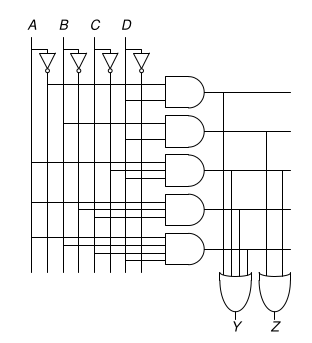
\includegraphics[width=0.5\linewidth]{image.png}
    \vspace{1em}
    \centerline{\textbf{Figura 2.} Circuito}
\end{figure}

\noindent\textbf{Ejercicio 7.} Minimiza la ecuación booleana del ejercicio 6 y diagrama un circuito mejorado que cumpla la misma función.

\vspace{0.5cm}

\noindent\textbf{Ejercicio 8.} Usando \textit{De Morgan} o \textit{Bubble Pushing}, redibuja el circuito de la figura 3 de modo tal que puedas encontrar la ecuación booleana del circuito. Escribe la ecuación booleana.

\begin{figure}[h]
    \centering
    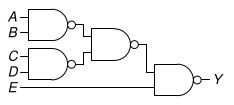
\includegraphics[width=0.5\linewidth]{image_2.png}
    \vspace{1em}
    \centerline{\textbf{Figura 3.} Circuito NAND}
\end{figure}

\pagebreak

\noindent\textbf{Ejercicio 9.} Repite el ejercicio 8 para la figura 4.

\begin{figure}[h]
    \centering
    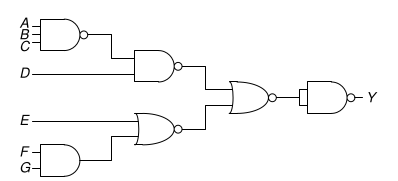
\includegraphics[width=0.75\linewidth]{image_3.png}
    \vspace{1em}
    \centerline{\textbf{Figura 4.} Circuito NAND y NOR}
\end{figure}

\noindent\textbf{Ejercicio 10.} Escribe una ecuación booleana minimizada para la función que realiza el circuito de la figura 5.

\begin{figure}[h]
    \centering
    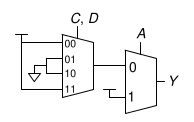
\includegraphics[width=0.5\linewidth]{image_4.png}
    \vspace{1em}
    \centerline{\textbf{Figura 5.} Circuito de multiplexores}
\end{figure}

\noindent\textbf{Ejercicio 11.} Implementa un circuito usando la tabla de verdad \textbf{(b)} de la Figura 1, usando:
\begin{enumerate}
    \item Un multiplexor 8:1.
    \item Un multiplexor 4:1 y una compuerta NOT.
    \item Un mulplexor 2:1 y dos compuertas lógicas.
\end{enumerate}

\pagebreak

\noindent\textbf{Ejercicio 12.} Determina el tiempo de propagación y el tiempo de contaminación del circuito de la figura 4. Utiliza los tiempos de retardo dados en la tabla 1.

\begin{figure}[h]
    \centering
    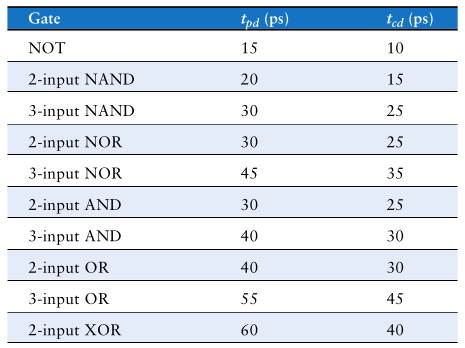
\includegraphics[width=0.75\linewidth]{image_5.png}
    \vspace{1em}
    \centerline{\textbf{Tabla 1.} Tiempos de retardo}
\end{figure}

\end{document}